\chapter{Overview of a DBMS}

This chapter will give a general overview of the structure of a centralized \textbf{DBMS} (\textbf{Data Base Management System}) based on the relational data model, describing its components and their respective functionalities.

\section{Architecture}

A database is a collection of homogeneous sets of data, with relationships defined among them, stored in permanent memory, and used via a DBMS.

\BoxDef{DBMS}{
A DBMS is a software that provides the following functionalities:
\begin{itemize}
    \item A language to describe the \textbf{schema} of the database (a collection of definitions that describe the data structures), restrictions on the allowed data types, and the relationships among data sets;
    \item The data structures for storage and efficient retrieval of large amounts of data;
    \item A language to guarantee secure access to the data only to authorized users;
    \item A \textbf{transactions} mechanism to protect data from HW/SW malfunctions and errors during concurrent access.
\end{itemize}
}

The architecture of a DBMS provides the following basic components:
\begin{itemize}
    \item The \textbf{Storage Engine}, which includes modules supporting:
    \begin{itemize}
        \item \textbf{Permanent Memory Manager};
        \item \textbf{Buffer Manager};
        \item \textbf{Storage Structures Manager};
        \item \textbf{Access Methods Manager};
        \item \textbf{Transaction and Recovery Manager};
        \item \textbf{Concurrency Manager}.
    \end{itemize}

    \item The \textbf{Relational Engine}, which includes modules supporting:
    \begin{itemize}
        \item \textbf{Data Definition Language};
        \item \textbf{Query Manager};
        \item \textbf{Catalog Manager}.
    \end{itemize}
\end{itemize}
In real systems the functionalities of these modules are not completely separated in different components (as in Figure \ref{fig:DBMS_schema}), but this overview can help in understanding the purpose of each of them. 

\begin{figure}[ht]
    \centering
    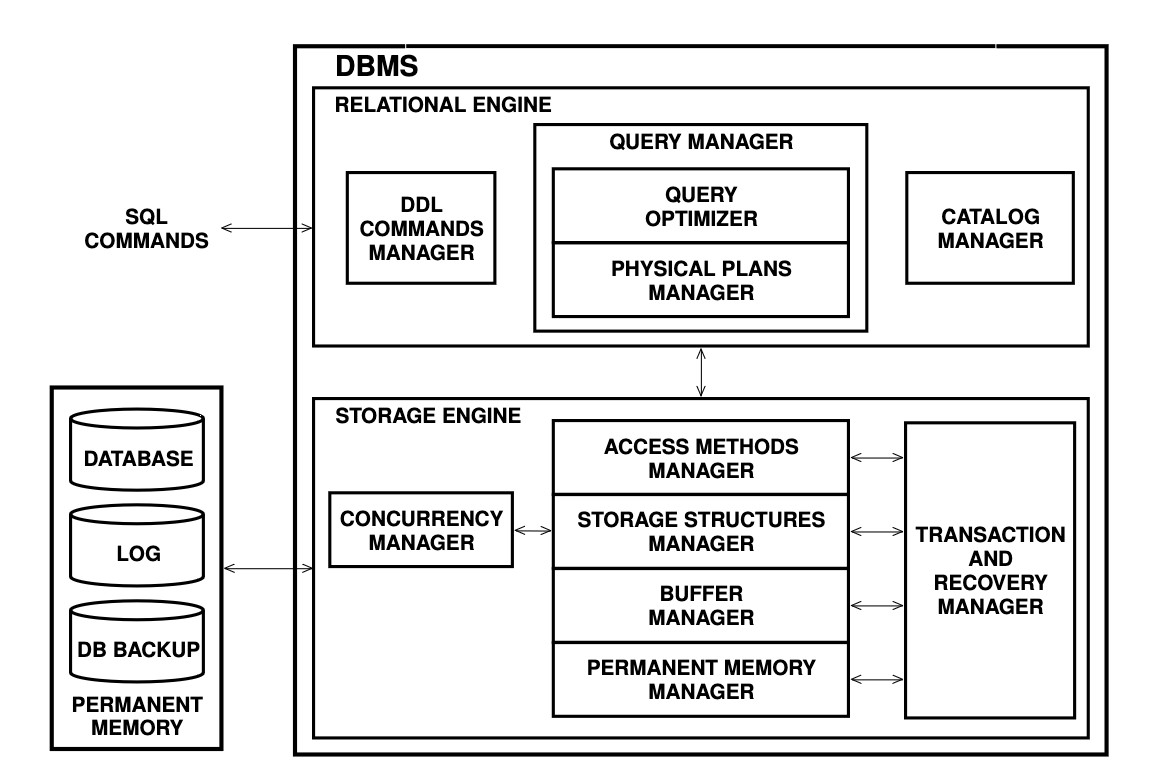
\includegraphics[width=0.75\linewidth]{img/DBMS schema.png}
    \caption{The architecture of a DBMS.}
    \label{fig:DBMS_schema}
\end{figure}

\subsection{Permanent Memory Manager}

The PMM manages page allocation and deallocation on disk storage. It hides the disk characteristics and the operating system, as it provides an abstraction of the memory as a a set of databases, each consisting of a set of logical files of \textbf{physical pages} (or blocks) of fixed size. The physical pages of a file are numbered consecutively starting from 0, and their number can grow dynamically with the only limitation being the available space in the permanent memory. Each collection of records (table or index) of a database is stored in a logical file, which can also be realized as an actual separate file of the operating system or as part of a file in which the database is stored.

Once a physical page is transferred to main memory, it is called a \textbf{page}, and it is represented with a specific, complex structure.

\subsection{Buffer Manager}

The Buffer Manager is tasked with transferring pages between temporary and permanent memory. It allows transactions to get the pages they need minimizing the number of disk accesses. In general, the performance of operations on a database depends on the number of pages transferred to temporary memory. If a big enough buffer is used, and there's a high number of access requests for a specific page, there's a high likelihood that such page will be in the buffer. Figure \ref{fig:buffermanager} illustrates the basic structure of a Buffer Manager.

\begin{figure}[ht]
    \centering
    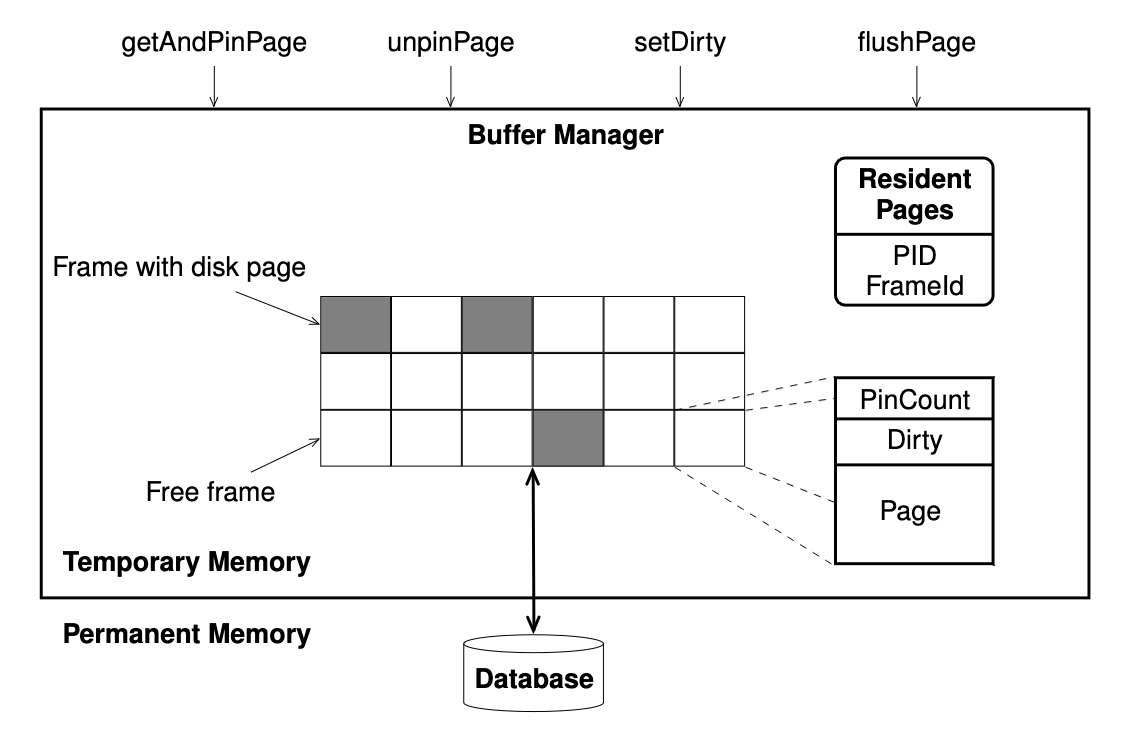
\includegraphics[width=0.5\linewidth]{img/Buffer Manager.png}
    \caption{The components of the Buffer Manager.}
    \label{fig:buffermanager}
\end{figure}

The \textbf{buffer pool} is an array of \textbf{frames}, each containing a copy of a page present in permanent memory, and some additional bookkeeping information. The pool has a fixed size, so when there are no more free frames, a page must be freed with an appropriate algorithm. Each frame stores two variables, the \textbf{pin count} and the \textbf{dirty}. The former counts the number of transactions currently using the page hosted on that frame; its value starts at 0, and increases by 1 each time it is requested, and decreases by 1 each time it is released. The latter indicates whether the page was modified since it was copied into the buffer, signaling that the modification must be reflected on disk as well. The \textbf{resident pages} table is a hash table that is used to know which page in permanent memory (identified by a PID) is stored in which frame.

A commonly used replacement policy is the \textbf{Least Recently Used} (\textbf{LRU}) policy. Once the buffer pool is full, the frame chosen to be ejected is the one that was the earliest one to be pinned. The idea is that since the page hasn't been requested for a relatively long time, it probably won't be requested any time soon. However, this policy may not always be the best: for example, in a join loop between two tables, the LRU policy may be optimal for one table, while the optimal one for the other is Most Recently Used (MRU).

\subsection{Storage Structures Manager}

The Storage Structure Manager implements databases as tables of records, representing the files of pages provided by the Permanent Memory Manager. Above the Storage Structure Manager, the unit of access is a record; below, the unit of access is a page. For this reason, the unit of costs considered for now will be a single page access (read or write), and we assume that memory operations have 0 cost, since they're so much faster than disk operations their addition to the overall cost is negligible. The most important type of file is the \textbf{heap file}, which stores records in no particular order.

A \textbf{record} is a collection of one or more \textbf{attributes}, and contains some extra information, called \textbf{record header}, needed for record management. We assume records are not larger than a page (a few KB big), and that each attribute is either separated from the others using a separator, or all attributes are stored sequentially and are indexed by using an offset. Each record is uniquely identified by a \textbf{RID}, which specifies the page and the offset the record can be found at. Sometimes this offset may be logical, i.e., it actually indicates a position on an array of actual pointers to records; this way, records can be moved around without having to externally modify their RID.

Collections of pages may be stored using different data structures. Usually, pages are stored with two alternatives. The first uses two doubly linked list, one containing free pages, the other containing full ones. The other alternative consists in a \textbf{directory}, where each entry contains a pair PID-available space. If the directory grows and cannot be stored in the header page of the file, it is organized as a linked list. For efficiency reasons, the free space existing in different spaces cannot be compacted into new free pages. If the available free space is plenty but there's no actual free pages available, it may be necessary to reorganize the database.

\section{External Sorting}

A frequent operation done in DBMS is \textbf{sorting}. Sorting collections of records may be done for different reasons: it may be needed to perform a join operation, delete duplicates, or load them into physical organizations.

Since typically temporary memory cannot hold all of the records of a file at the same time, merging is done by using \textbf{external sorting algorithms}, of which most widely used one is \textbf{merge-sort}. Let $N_{pag}(R)$ be the number of pages in the file, and $B$ the number of available pages on the buffer. Merge-sort operates in two phases:
\begin{enumerate}
    \item The \textbf{sort phase}, in which $B$ pages are read into the buffer, sorted, and written to disk. This creates exactly $n = \ceil{N_{pag}(R) / B}$ sorted subsets of records, called \textbf{runs}. Each run is stored in a separate numbered auxiliary file, and contains the same number of pages (except for the last one, which may contain less if the number of file pages isn't divisible by the number of free buffer pages);

    \item The \textbf{merge phase}, which fuses the sorted runs to reconstruct the file. In each merge pass, $Z = B-1$ runs are merged using one buffer page left free to produce the output. The number of runs at the end of a merge pass becomes $n = \ceil{n/Z}$. Merges are repeated until $n < 1$.
\end{enumerate}
Once the algorithm terminates, the final auxiliary file contains the sorted data. $Z$ is called the \textbf{merge order}, and a total of $Z + 1$ buffer pages are needed to execute a $Z$-merge (since as stated above, one page must be left free).

The cost of the algorithm is evaluated in terms of how many read/write operations are needed in total, since we're ignoring operations directly involving records. The overall cost is given by two terms:
\begin{align*}
    C_{sort}(R) = SortCost + MergeCost = \\
    = 2 \times N_{pag}(R) + 2 \times N_{pag}(R) \times MergePasses
\end{align*}
If the number of file pages is less than $B^2$, (or, more precisely, $B(B-1)$), the data can be sorted in a single pass, so the cost becomes:
\begin{equation*}
    C_{sort} = 2 \times N_{pag}(R) + 2 \times N_{pag}(R) \times 1 = 4 \times N_{pag}(R)
\end{equation*}
The number of passes is a function of the number of file pages $N_{pag}(R)$, the number of initial runs $S$, and $Z$. $S$ also depends on the number of file pages and the number of buffer pages available at the start:
\begin{equation*}
    S = \ceil{N_{pag}/B}
\end{equation*}
At each merge pass, the algorithm merges together $Z$ runs. At the start, the runs will be $S$. After one merge pass, they will be $S/Z$. At the second pass, they will be $S/Z * 1/Z = S/Z^2$, and so on until only one run remains. Since the number of runs decreases exponentially, we can write that the total number of passes will be:
\begin{equation*}
    k = \ceil{\log_Z{S}}
\end{equation*}
The total cost can be rewritten as:
\begin{equation*}
    C_{sort} = 2 \times N_{pag}(R) + 2 \times N_{pag}(R) \times \ceil{\log_Z(S)} \ .
\end{equation*}

\section{Data Organizations}

\subsection{Heap and Sequential Organizations}

The data can be arranged either via \textbf{heap organization}, or \textbf{sequential organization}. With heap organization, every new record is added to the end of the file: insertion is easy and efficient in terms of memory used. It is ideal for situations where insertion is more common than search, or files where massive search is common. This is also the standard organization for DBMS.

With sequential organization, data is kept sorted on a \textbf{search key} $K$, picked as a single attribute of the records. This makes equality and range search on $K$ very efficient. On the other hand, insertion is more problematic, since the ordering of the records must be maintained at all times. Insertion may use a \textbf{static solution}, where each page is filled normally, and for each insertion, the record is placed at the correct spot in the ordering, moving all other records after it. A \textbf{dynamic solution} instead keeps some fraction of the total space in a page free. Once a page has filled up enough, its contents are split into new pages. This way, pages always have some extra space at the end to accommodate new insertions: when a record is added, the shifting of the records after it will only involve the ones in the same page. Alternatively, a \textbf{differential file} may be used to keep track of which changes must be applied to which pages, so that all insertions can be done all at once in a second moment.

Table \ref{tab:heap-seq-comp} shows a comparison between the two organization types. $N_{pag}(R)$ refers to the number of pages required to store the records. The \textbf{selectivity factor} $sf$ is an estimate of the fraction of pages occupied by records that satisfy the condition of a range search, and is calculated as:
\begin{equation*}
    sf = \dfrac{(k_2 - k_1)}{(k_{max} - k_{min})} \ ,
\end{equation*}
with $k_1$ and $k_2$ being the two extremes of the range, and $k_{max}$ and $k_{min}$ the highest and lowest values in the domain of the attribute.

\begin{table}[ht]
\small
\centering
\SetTblrInner{rowsep=5pt}
\begin{tblr}{hlines, vlines, columns={75pt, c, m}, column{1}={50pt, c}, column{2}={50pt, c}, column{5}={50pt,c}, column{6}={50pt, c}}
        \textbf{Type} & \textbf{Memory} & \textbf{Eq. Search} ($C_s$) & \textbf{Range Search} & \textbf{Insertion} & \textbf{Deletion} \\
\hline
        \textbf{Heap} & $N_{pag}(R)$ & $\ceil{\dfrac{N_{pag}(R)}{2}}$ & $N_{pag}(R)$ & $2$ & $C_s + 1$ \\

        \textbf{Seq.} & $N_{pag}(R)$ & $\ceil{\log_2{N_{pag}(R)}}$ & $C_s - 1 + \ceil{sf \times N_{pag}(R)}$ & $C_s + 1$ $+ N_{pag}(R)$ & $C_s + 1$ \\

\end{tblr}
    \caption{Comparison between heap and sequential organization.}
    \label{tab:heap-seq-comp}
\end{table}

The equality search is faster for the sequential one since it uses a binary search algorithm, while the heap one has to compare the record against all pages since no specific ordering is imposed. The cost estimation is also only valid if the data distribution is uniform; if it follows some other distribution, e.g., Gaussian, the actual cost may be high (worst case exactly $N_{pag}(R)$).

The range search for the heap organization costs $N_{pag}(R)$ since it must read all pages to make sure it collects all records falling within the specified range. For sequential organization, it costs an equality search to find the starting record of the range, plus the number of pages needed to store the records in that range. The ``$-1$'' is added because the first page has already been found with the binary search.

The final biggest difference lies in the costs for insertions: it is constant for heap organization, while for sequential organization it costs a search to find the spot to insert the record, and all subsequent $N_{pag}/2$ pages must be read and written to move their records forward. If the page the record is added to is not completely full, the insertion will still cost $C_s + 1$.

\subsection{Key-based Organizations}

A table organization based on a key allows the retrieval of a record with a specified key in as few accesses as possible, 1 being the optimum. The set of records in the table is \textbf{mapped} to a set of keys, via either a \textbf{primary organization} or a \textbf{secondary organization}.
\BoxDef{Primary and Secondary Organizations}{
A table organization is primary if it determines the way the records are physically stored, and therefore how they can be retrieved. Otherwise, it is a secondary organization.
}
For a primary organization, the mapping can be done using a \textbf{hash function} or a \textbf{tree structure}. It can be either \textbf{static} or \textbf{dynamic}.
\BoxDef{Static and Dynamic Primary Organization}{
A primary organization is static if the performance degrades gradually as insertions and deletions are performed, requiring reorganization. \\
A primary organization is dynamic if once created, it evolves with insertions and deletions, preserving efficiency of operations.
}
In a secondary organization, the mapping from key to record is implemented with the \textbf{tabular method}/\textbf{index}, listing all inputs and outputs.

\subsubsection{Static Hashing Organization}

This is the simplest methods for a primary table organization. We assume to have $N$ records all of the same fixed size, and that keys are integers. The records of the same table $R$ are stored in the \textbf{primary area}, divided into $M$ buckets, each of which may consist of one or several pages. For now, we will assume each bucket to contain only one page of capacity $c$, and that pages are numbered from $0$ to $M-1$.

A record is inserted into a specific bucket chosen by calculating its address via a \textbf{hashing function} $H$, applied to the record key value. The ratio:
\begin{equation*}
    d = \dfrac{N}{(M \times c)}
\end{equation*}
is called the primary area \textbf{loading factor}, which represents how full the primary area is. The hash function should produce addresses uniformly distributed in the interval $[0, M-1]$, and it may return the same address for different keys. This causes a \textbf{collision}. Records hashed to the same page are stored in order of insertion. When an insertion is attempted in a page that is completely full, an \textbf{overflow} occurs, and must be appropriately managed.

The design of a static hashing organization depends on the choices done for the following parameters:
\begin{enumerate}
    \item The \textbf{hashing function}: a good hashing function must randomly assigning keys to elements in the address space. There's no single ``ideal'' hash function, but generally, simpler functions tend to perform better than complex ones. A common choice is the \textbf{modulo function}: $H(k) = k \mod M$, with $M$ a prime number.

    \item The \textbf{overflow management technique}: two commonly used techniques are \textbf{open overflow} and \textbf{chained overflow}. Open overflow performs a primary area linear search to find the first empty space to insert the record; when the last page has been searched, the process restarts from the initial page. Chained overflow collects overflow records chained together in a separate area, pointed to from the home page.

    \item The \textbf{loading factor}: low loading factors and higher page capacities give better performances, but occupy more memory. For low ($d < 0.7$) loading factors, retrieving a record requires a single access on average. For high values ($d > 0.8$), the primary area size is reduced, increasing the probability of overflow; open overflow deteriorates rapidly, while chained overflow still performs well.  

    \item The \textbf{page capacity}: higher values of page capacity reduce the number of overflows, which are the main culprit in performance degradation of hashing organizations.
\end{enumerate}
As for overall performances, for page capacities less than 10 it is preferable to give up hash organizations. A static hashing has excellent performances as long as there are no overflows to manage, with the average cost of an equality search being 1. As overflows start to happen, reorganization is needed, which requires the creation of a new primary area, choosing a new hash function, and reloading all the data.

A big drawback of static hashing is that is does not support efficient range queries, since records with similar keys will typically not end up in the same bucket.

\subsubsection{Dynamic Hashing Organization}

Dynamic hashing organizations can be divided into two groups: those that use a primary area and an auxiliary data structure whose size changes with the primary area size, and those in which only the primary area size changes dynamically. In both cases, the hashing function changes automatically when the structure changes dimension, maintaining the average access time equal to 1. We will see two types of dynamic organizations with auxiliary data structures (Virtual Hashing and Extendible Hashing), and two without (Linear Hashing and Spiral Hashing).

\paragraph{Virtual Hashing}

Virtual hashing works as follows:
\begin{enumerate}
    \item The data area initially contains $M$ contiguous pages of capacity $c$. Each page is identified by its address (between $0$ and $M-1$).

    \item A bit vector $\mathcal{B}$ is created, indicating with a $1$ which page contains at least a record.

    \item An initial function $H_0$ is used to map each key to and address $m$. If an overflow happens, then the data area is doubled, maintaining the pages as contiguous, the hashing function is replaced with a new one ($H_1$) that maps keys to addresses in the range $[0, 2M-1]$, and the hashing function is applied to all keys and all records in the overflowing page $m$. These records end up being distributed between $m$ itself and some other new page $m'$.
\end{enumerate}
This method defines a series of hashing functions,
\begin{equation*}
    H_0, H_1, H_2, \dots, H_r \ ,
\end{equation*}
where $H_i$ produces a page address in the range $[0, 2^i M-1]$. The function chosen as the hash function must satisfy the following constraints:
\begin{align*}
    &H_{j+1}(k) = H_j(k) \\
    \text{or}\\
    &H_{j+1}(k) = H_j(k) + 2^j \times M ,\ j=r,r-1,\dots,0
\end{align*}
for all keys $k$. This means that the new hash function chosen either returns the same address the key already corresponds to, or a new address that is equal to the original one plus half of the new address space. A common function is $H_r(k) = k \mod (2^r \times M)$.

To find a record, known its key and $r$ (the number of times the data area has been doubled), a recursive function is used:
\begin{algorithm}[ht]
\caption{PageSearch pseudocode.}
\begin{algorithmic}[1]
    \If{$r < 0$}
        \State The key does not exist.
    \ElsIf{$\mathcal{B}(H_r(k)) == 1$}
        \State Return $H_r(k)$
    \Else
        \State PageSearch($r-1$, $k$)
    \EndIf
\end{algorithmic}
\end{algorithm}
This technique requires memory equal to the one occupied by the data area and the bit vector $\mathcal{B}$. The memory is not very well used however, because of the frequent need to double the data area.

\paragraph{Extendible Hashing}

Instead of using a bit vector, extendible hashing uses a fixed set of data pages with a \textbf{directory} $\mathcal{B}$, containing a set of pointers to data pages. The directory is smaller in size than the primary area, and is doubled as needed.

Let $r$ be a record with key $k$. The value produced by $H(k)$ is a binary value of $b$ bits (usually 32), called hash key. The hash key does not represent an actual address; instead, pages are allocated on demand as records are inserted into the file, considering only the initial $p$ bits of $b$, which are used as an offset into the directory $\mathcal{B}$. The value of $p$ grows and shrinks with the number of pages used by data, and the number of entries in the directory is always $2^p$. $p$ is called the \textbf{directory level}. Each entry in the directory is a pointer to a data page containing records with the same first $p'$ bits of their hash key, with $p' \in [0, p]$. $p'$ is called \textbf{data page level}.

The hash structure is initially empty, with $p=0$, and is a directory with one entry containing a pointer to an empty page of capacity $c$. The first $c$ records are inserted in the page; as we try to insert a new record into a full page, there are two possibilities:
\begin{itemize}
    \item If $p' = p$, $\mathcal{B}$ is doubled and $p$ becomes $p+1$. Let $w$ be the bits of the previous value of $p$. Then, the entries in the doubled directory indexed by $w0$ and $w1$ each contain a pointer to the same data page that $w$ used to point to.

    \item If $p' < p$, then the data page is split in two, creating a new page, and each of the halves' level $p'$ take value $p'+1$. The records in the original page are distributed across the halves, based on the value of the first high-order bit of their hash keys. Records whose key has 0 in the $(p'+1)^{th}$ bit stay in the old page, while those with a 1 will go in the new one. The pointers in the directory are updated so that those that pointed to the original page now point to the new half, depending on the value of the $(p'+1)^{th}$ bit.
\end{itemize}
The advantage of this method is that performance does not degrade as the file grows, and the directory $\mathcal{B}$ keeps the memory overhead low. The retrieval of a record has an additional level of indirection since $\mathcal{B}$ must be accessed first, but this has very little impact on the performance, since most of the directory will be in main memory.

\paragraph{Linear Hashing}

Linear hashing increases the number of data pages as soon as an overflow occurs, but the page which is split is not the one that flows over; instead, it is the page pointed by the current pointer $p$, initially equal to 0, and incremented to 1 each time an overflow happens.

Initially, $M$ pages are allocated, and the hash function used is $H_0(k) = k \mod M$. When an overflow happens in a page with address $m \geq p$, an overflow chain is maintained for page $m$, and a new page is also added. All records in page $p$ are distributed between page $p$ and the new page, using the new hash function $H_1(k) = k \mod 2M$.

As page $M$ overflows, a total of $M$ duplications have happened, bringing the memory to $2M$ pages. Pointer $p$ is reset, and $H_0$ is replaced by $H_1$. $H_1$ is in turn replaced by $H_2(k) = k \mod 2^2 M$, and so on. After $r$ doublings, the function $H_r(k) = k \mod 2^r M$ will be used. To retrieve a record with key value $k$, the page address is calculated as:
\begin{algorithm}
\caption{PageAddress pseudocode.}
\begin{algorithmic}[1]
    \If{$H_i(k) < p$}
        \State $H_{i+1}(k)$
    \Else  
        \State $H_i(k)$
    \EndIf
\end{algorithmic}
\end{algorithm}
\\Linear hashing has similar performances to extendible hashing.

\paragraph{Spiral Hashing}

Spiral hashing considers the memory as if it were organized on a spiral instead of a line. Like linear hashing, spiral hashing requires no index, but has better performances and storage utilization because of three particular property:
the hashing function distributes records unevenly, accumulating records in the pages at the beginning of the address space, while the pages at the end have a lower load. The page that is split is one that is very unlikely to overflow.

\subsubsection{Tree-structure Organizations}

All the previous organizations have the big disadvantage of not supporting the range equality search operation. An alternative organization commonly used in DBMSs use dynamic tree structures to store pages. The \textbf{order} of a tree is the maximum number of children a node can have. The \textbf{level} of a node is the number of nodes encountered in the path from the root to the node itself. The \textbf{height} of the tree is the maximum level of a node. A tree is \textbf{balanced} if the levels of all leaf nodes differ by at most 1.

The types of trees most commonly used are B-trees and B$^+$-trees, since unlike binary trees they manage to keep a relatively low height even with an high number of pages. One solution may be to store the nodes of the binary tree in main memory, such that each page contains the same number of nodes. In the example shown in Figure \ref{fig:paged-bintree}, each page contains 8 nodes, each of which refers to 8 different pages. Using this strategy, the depth of the tree in terms of pages to access is greatly reduced: an equality search has a complexity of $\log_8 (N_{pag}(R))$ instead of $\log_2 (N_{pag}(R))$.

\begin{figure}[h!]
    \centering
    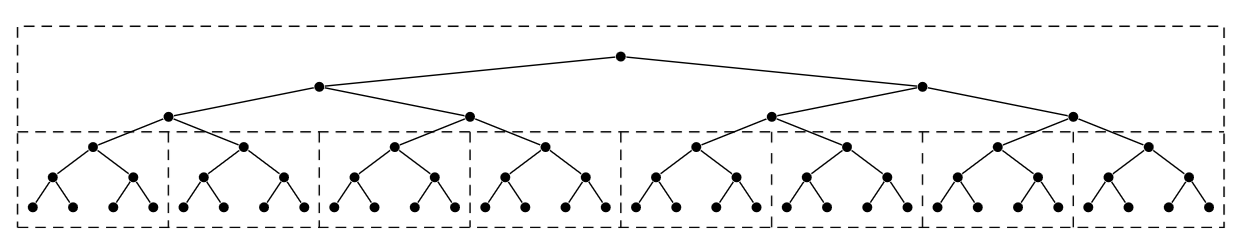
\includegraphics[width=1.0\linewidth]{img/paged_bintree.png}
    \caption{A paged binary tree: each page in main memory is delimited by a dashed line.}
    \label{fig:paged-bintree}
\end{figure}

Still, this structure must be kept balanced when insertions or deletions are performed, and algorithms that maintain binary trees can be very costly. The following sections will explain how using multiway trees can be a solution.

\paragraph{B-trees}

A B-tree is a perfectly balanced search tree, in which each node has a variable number of children. We will indicate a key as $k$ and the full record associated with it $k*$. Also, we'll assume that all keys are integers and that all records have the same fixed size. An example of B-tree can be seen in Figure \ref{fig:B-tree}.

\begin{figure}[ht]
    \centering
    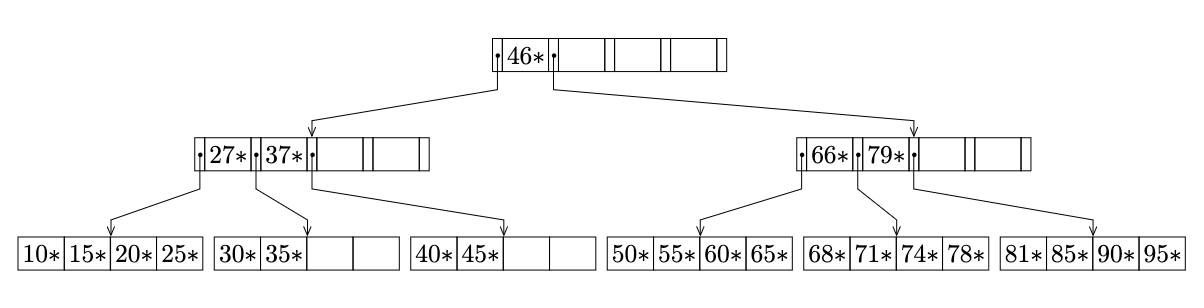
\includegraphics[width=1.0\linewidth]{img/B-tree.png}
    \caption{A B-tree.}
    \label{fig:B-tree}
\end{figure}
A B-tree is defined as follows:
\BoxDef{B-tree}{
A B-tree of order $m \geq 3$ is an $m$-way search tree that is either empty or of height $h \geq 1$, and satisfies the following properties:
\begin{itemize}
    \item Each node has at most $m - 1$ keys, and, except for the root, at least $\ceil{m/2} - 1$ keys;

    \item A node with $j$ keys will have $j+1$ pointers to children, undefined in the leaves, and $K(p_i)$ is the set of all keys in the $i^{th}$ child node;

    \item All leaves are on the same level;

    \item Each non-leaf node has the same following structure:
    \begin{equation*}
        [p_0, k_1*, p_1, k_2*, \dots, k_j*, p_j] \,,
    \end{equation*}
    where each $p_i$ is a pointer to a child node such that, for all $0 < i < j$:
    \begin{align*}
        &\forall k \in K(p_i), \ k_{i} < k < k_{i+1}
    \end{align*}
\end{itemize}
}
There is a strict relationship between the height of the tree $h$, the order $m$, and the number of keys $N$. Since the non-root nodes are constrained in the number of keys they must maintain, the following inequality holds true:
\begin{equation*}
    \log_m (N+1) \leq h \leq \log_{\ceil{m/2}}(\dfrac{N+1}{2}) + 1
\end{equation*}
The left size of the inequality corresponds to a B-tree with all of its nodes completely filled, while the right side to a B-tree where each node has the least acceptable amount of keys.

The following is a summary of the costs of operations using a B-tree. An equality search for a specific key $k$ starts at the root; if the key is not in the root (and $h > 1$), the search continues in the child that will likely contain the key (since keys are ordered, the chosen pointer is the one right after the biggest key smaller than $k$). The overall cost is $1 \leq C_s \leq h$.

As for the range search, to retrieve all records with keys in increasing order, the tree must be visited in the \textbf{in-order traversal}, starting from the leftmost leaf and gradually moving to the right. Let $sf = (k_2 - k_1)/(k_{max} - k_{min})$ be the selectivity factor for the search; the overall cost will be $C_{range} = sf \times N_{nodes}$, since keys will be ``scattered'' across different nodes of the tree at different levels. The following bond holds true: $h \leq C_{range} \leq N_{nodes}$. It will always require traveling to a leaf, and in the worst case scenario, it may have to read all nodes in the tree.

Insertion in a non-full leaf is easy: the new key is simply added to a leaf so that the keys are correctly sorted. The cost is $h$ reads and 1 write. If the leaf is full, then the node must be split, so that the old node will retain the first half of keys, and the new node will get the second half. The median key is inserted into the parent node, and the new node is pointed by the pointer on its right. In case the parent node is full as well, the operation repeats. The cost for a worst case scenario is $h$ reads and $2h + 1$ writes.

For deletion, there's three possibilities:
\begin{itemize}
    \item If the key is in a leaf, and the removal keeps the number of keys within the acceptable range, the cost is $h$ reads and 1 write;

    \item If the key is a node, and no other operations are needed, the cost is $h$ reads and 2 writes (the key is replaced with the next following one);

    \item If the key is in a leaf node and the final number of keys is less than $\ceil{m/2} - 1$ elements, then a \textbf{rotation} or a \textbf{merge} are needed.

    A node is merged with one of its brothers which contains $\ceil{m/2} - 1$ keys, moving all of them to the first node. Additionally, the key in the parent node that was between the pointers of the two children involved in the merging is also removed and added to the merged child. In case this produces an underflow in the parent node, the operation is repeated until the whole tree is balanced.

    When a merge is not possible because all brothers are too full, a rotation is performed instead. When the key is deleted, the maximum key from the left brother is moved into the parent, and the key in the parent is moved into the underfull node.

    When either of these operations are needed for all nodes from root to leaf, the cost is $2h - 1$ reads and $h + 1$ writes.
\end{itemize}
Table \ref{tab:B-tree-comp} summarizes all the operation costs.

\begin{table}[ht]
\small
\centering
\SetTblrInner{rowsep=5pt}
\begin{tblr}{hlines, vlines, columns={80pt, c, m}, column{1}={60pt}}
    & \textbf{Eq. Search} ($C_s$) & \textbf{Range Search} & \textbf{Insertion} & \textbf{Deletion} \\
\hline
    Best case & 1 & $sf \times N_{nodes} = h$ & $h + 1$ & $h + 1$ or $(h + 2)$ \\     
    Worst case & $h$ & $sf \times N_{nodes} = N_{nodes}$ & $2h + 1$ & $(2h - 1) + (h + 1)$ \\
\end{tblr}
    \caption{Costs for B-tree organization.}
    \label{tab:B-tree-comp}
\end{table}

\paragraph{B$^+$-trees}

B$^+$-trees are a variant of B-trees that perform especially well for range searches. In a B$^+$-tree, all the records $k*$ are stored sorted in the leaf nodes, organized in a doubly linked list. Each non-leaf node stores the highest key of the child pointed by the previous pointer. An example of B$^+$-tree can be seen in Figure \ref{fig:B+-tree}.

\begin{figure}[ht]
    \centering
    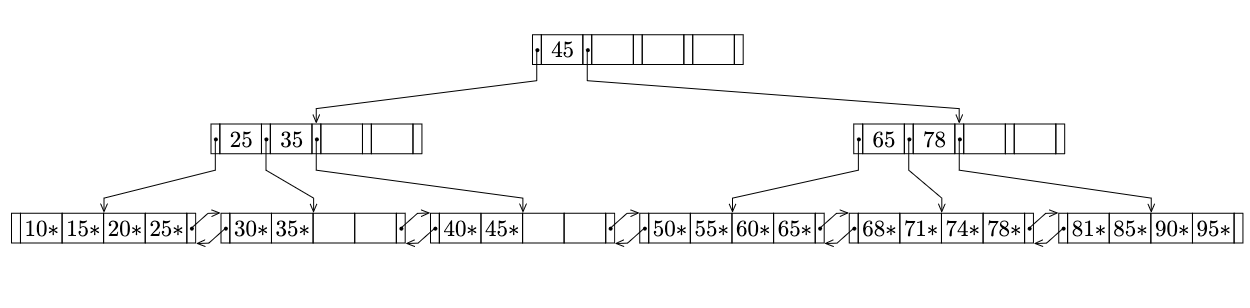
\includegraphics[width=1\linewidth]{img/B+-tree.png}
    \caption{A B$^+$-tree.}
    \label{fig:B+-tree}
\end{figure}
It can be thought of as the combination of a sparse index and a sequential file. Records are part of the tree structure stored in one file, so to read all records in a sorted order, the tree structure must be necessarily used to locate the first data page.

Compared to B-trees, B$^+$-trees tend to be much shallower, since the non-leaf nodes only contain keys but not records, which can be found in the leaves, connected together. This makes any sequential/range scan of the data faster: the cost for a ranged search is $sf \times N_{leaves}$. For the equality search, since we're assuming the tree to have a level equal to no more than 3, will take from 1 to 3 read operations.

Another big difference is that in deletion, there's no need to replace it in the father node, unless the deletion requires a merge or rotation (in which case the operations are the same as the B-tree).

\subsubsection{Index (Secondary) Organizations}

A secondary organization is defined as follows:
\BoxDef{Secondary Organization}{
An index $I$ on a key $K$ of a set of records $R$ is a sorted table $I(K, RID)$ on $K$, where $N_{rec}(R) = N_{rec}(I)$. An element of the index is a pair $(k_i, r_i)$, where $k_i$ is the key of a record, and $r_i$ is the corresponding RID.
}
An index is a tabular data structure that supports fast retrieval of records by exploiting the ordering of the keys. It can be defined on one or more keys. An index is typically stored in a B$^+$-tree structure.

If the order of the data records is approximately the same as the order of the entries in the index, then it is called a \textbf{clustered index}. When the index is first created, a sort is performed on the actual data records, matching the index order. As insertions are performed, this ordering may be gradually lost, also reducing the effectiveness of such organization, so the clustered index may have to be recreated from time to time. If instead the data records do not follow the same order as the index records, it is called an \textbf{unclustered index}.

The cost for searches done using this organization can be broken down into two terms:
\begin{equation*}
    C_s = C_I + C_D \,,
\end{equation*}
where $C_I$ is the cost of accessing the index pages to find the $RID$s needed, and $C_D$ is the cost of accessing the actual data pages containing the records. Table \ref{tab:indexes-comp} summarizes the differences between the two types of indexes.

\begin{table}[ht]
\small
\centering
\SetTblrInner{rowsep=5pt}
\begin{tblr}{hlines, vlines, columns={80pt, c, m}}
    & \textbf{Eq. Search} ($C_s$) & \textbf{Range Search} \\
\hline
    Clustered & $C_I = 1$, $C_D = 1$ & $C_I = sf \times N_{leaf}$, $C_D = sf \times N_{pag}$ \\     
    Unclustered & $C_I = 1$, $C_D = 1$ & $C_I = sf \times N_{leaf}$, $C_D = sf \times N_{rec}$ \\
\end{tblr}
    \caption{Costs clustered vs. unclustered indexes.}
    \label{tab:indexes-comp}
\end{table}
In ranged search, both types need the same time to retrieve the relevant indexes: either way, they are always sorted by key and easily accessed since they're all part of the same doubly linked list; we're still assuming that since a B$^+$-tree structure is used, the tree will be pretty shallow. Using clustered indexes, the order in which indexes are found is the same as the order of the actual data on disk: the cost of accessing the data depends only on the number of pages the file is made up of, and we will only have to access $sf$ of them in order. With unclustered indexes, the data is not ordered in the same way as the index. There's no way to know exactly where each record is stored in relation to the pages, so each $RID$ returned by the key retrieval corresponds to an individual page access.

\subsection{Non-Key Attribute Organizations}

Up until now, all operations were done on keys, i.e., attributes that uniquely identify records. In many cases, however, we may be interested in retrieving records based on the values taken by other attributes. For example, imagine a table representing students attending the same school, each uniquely identified by a numeric code, and containing information about their name and age. An operation we may want to find all students within a specific age range, or all students who share the same surname. This section will describe how such operations can be done efficiently.

Specifically, the three types of operations that can be performed on non-key attributes are the equality search, the range search, and the \textbf{boolean search}, which consists in the previous operations combined together with boolean logical operators.


\subsubsection{Inverted Indexes}

\BoxDef{Inverted Index}{
An inverted index $Idx$ on a non-key attribute $K$ of a table $R$ is a sorted collection of entries, each in the form
\begin{equation*}
    (k_1, n, p_1, p_2, \dots, p_n) \,,
\end{equation*}
where each value $k_i$ of $K$ is followed by the number of records $n$ with that value, and the \textbf{sorted} RID list of these records.
}

Each entry in the inverted index has variable length, depending on how many records in the table $R$ have the same value for the attribute. Also, RIDs are added or removed as records are added or removed from the table. Despite the need to manage these indexes, they are still widely used, especially for cases in which searches are more common than insertions of deletions.

To evaluate performances, we will introduce these terms: $N_{key}(Idx)$ and $N_{leaf}(Idx)$, which are the number of distinct keys and leaf nodes in the index $Idx$. Also, all estimates are done assuming that index-key values are uniformly distributed, as well as records, and the index organization is a B$^+$-tree with the RID lists stored in the leaves. Each cost will be broken down into $C_I$ and $C_D$, as seen before.

For the equality search, the cost of accessing the index is simply $sf(\psi) \times N_{leaf}(Idx)$, or, alternatively, $\ceil{N_{leaf}(Idx) / N_{key}(Idx)}$. Here, $sf$ is calculated as:
\begin{equation*}
    sf(\psi) = \dfrac{1}{N_{key}(Idx)} \,,
\end{equation*}
since we're assuming uniform distribution of the values. All RIDs can be found close together since the leaves are sorted by key (i.e., the non-key attribute of the original table).

For $C_D$, the cost is different whether the data is sorted or not on the index key, so whether the index is clustered or unclustered. If it is unclustered, the operation must read all relevant records with no way to estimate where they are; for each record, the whole page must be read. Potentially, we may need to read an entire RID list worth of records, whose size is given by:
\begin{equation*}
    E_{rec} = sf(\psi) \times N_{rec}(R) = \ceil{\dfrac{N_{rec}(R)}{N_{key}(Idx)}}
\end{equation*}
The cost of retrieving the data is:
\begin{equation*}
    C_D = \ceil{\Phi(E_{rec}, N_{pag}(R))} \,,
\end{equation*}
where $\Phi()$ is called \textbf{Cardenas' formula}, and is estimated as:
\begin{equation*}
    \Phi(k,n) = n(1 - (1 - \dfrac{1}{n})^k) \leq \min(k,n)
\end{equation*}
So, the cost will be less or equal than the smallest term: if there's a lot more records than pages, chances are that a single page may contain multiple relevant records, while if the number of records is lower than that of pages, records will rarely appear together in the same page. If the index is clustered, then the cost is:
\begin{equation*}
    C_D = \ceil{sf(\Psi) \times N_{pag}(R)} 
\end{equation*}
Also, if the RID lists are unsorted, then the cost is always $E_{rec}$.

For the range search, $C_I$ remains the same, except that $sf(\Psi)$ is calculated as the ratio between the interval and the attribute's range. $C_D$ is calculated as the product between the number of index key values, and the number of pages to access to retrieve the records indicated by the RID lists. The first term is $\ceil{sf(\Psi) \times N_{key}(Idx)}$, because we will retrieve a certain number of records for each index key included in the range. The second term again depends on whether the index is clustered or unclustered.

If the index is unclustered, then $C_D$ is estimated as:
\begin{equation*}
    C_D = \ceil{sf(\Psi) \times N_{key}(Idx)} \times \ceil{\Phi(\ceil{\dfrac{N_{rec}(R)}{N_{key}(Idx)}}, N_{pag}(R))} \,,
\end{equation*}
while, if it is clustered, it is:
\begin{equation*}
    C_D = \ceil{sf(\Psi) \times N_{key}(Idx)} \times \ceil{\dfrac{1}{N_{key}(Idx)} \times N_{pag}(R)} = \ceil{sf(\Phi) \times N_{pag}(R)}
\end{equation*}
If the RID lists are unsorted, then the second term is always $\ceil{N_{rec}(R) / N_{key}(Idx)}$.

The summary of performances is shown in Table \ref{tab:inverted-idx}.

\begin{table}[ht]
\small
\centering
\SetTblrInner{rowsep=5pt}
\begin{tblr}{
    hlines,
    vlines,
    columns={160pt, c, m},
    column{1}={80pt}
}
     & \textbf{Eq. Search} & \textbf{Range Search} \\
    \hline
     Sorted RID lists, clustered & $C_I = $ as above, $C_D = \dfrac{1}{N_{key}(Idx)} \times N_{pag}(R)$ & $C_I = $ as above, $C_D = sf(\Psi) \times N_{pag}(R)$ \\
     Sorted RID lists, unclustered & $C_I = \dfrac{1}{N_{key}(Idx)} \times N_{leaves}(Idx)$, $C_D = \Phi(E_{rec}, N_{pag})$ & $C_I = \dfrac{v2 - v1}{v_{max} - v_{min}} \times N_{leaves}(Idx)$, $C_D = sf(\Psi) \times N_{key}(Idx) \times \Phi(E_{rec}, N_{pag}(R))$ \\
     Unsorted RID lists & $C_I = $ as above, $C_D = E_{rec}$ & $C_I = $ as above, $C_D = sf(\Psi) \times N_{key}(Idx) \times E_{rec}$ \\
    
\end{tblr}
\caption{Costs for inverted indexes.}
\label{tab:inverted-idx}
\end{table}

\subsubsection{Bitmap Indexes}

\BoxDef{Bitmap Index}{
A bitmap index $Idx$ on a non-key attribute $K$ of a table $R$ with $N$ records, is a sorted collection of entries in the form $(k_i, B)$, where each $k_i$ of $K$ is followed by a sequence of $N$ bits such that the $j^{th}$ bit is set to 1 if the $j^{th}$ record has value $k_i$ for attribute $K$, 0 otherwise.
}
Bitmap indexes are used in DBMS where data is never updated, such as data warehouses, since operations that modify this type of index can be complex, especially when it's compressed. They can also easily solve multi-attribute queries, since the answer can be found by doing a bit-wise AND between two or more bitmaps.

Indicating with $L_k$ and $L_{RID}$ the amount of bytes needed to store a key $k$ and a $RID$, and $D_{pag}$ the page size of the leaves, the number of leaves of a full inverted index is:
\begin{equation*}
    N_{leaf} = \dfrac{N_{key} \times L_k + N_{rec} \times L_{RID}}{D_{pag}} \approx \dfrac{N_{rec} \times L_{RID}}{D_{pag}}
\end{equation*}
while the number of leaves for a bitmap index is:
\begin{equation*}
    N_{leaf} = \dfrac{N_{key} \times L_k + N_{key} \times N_{rec}/8}{D_{pag}} \approx N_{key} \times \dfrac{N_{rec}}{D_{pag} \times 8}
\end{equation*}
Using these approximations, if the number of distinct values of the attribute is low, then a bitmap index is more convenient than an inverted index (as seen in Figure \ref{fig:bitmap-vs-inverted}). 

\begin{figure}[ht]
    \centering
    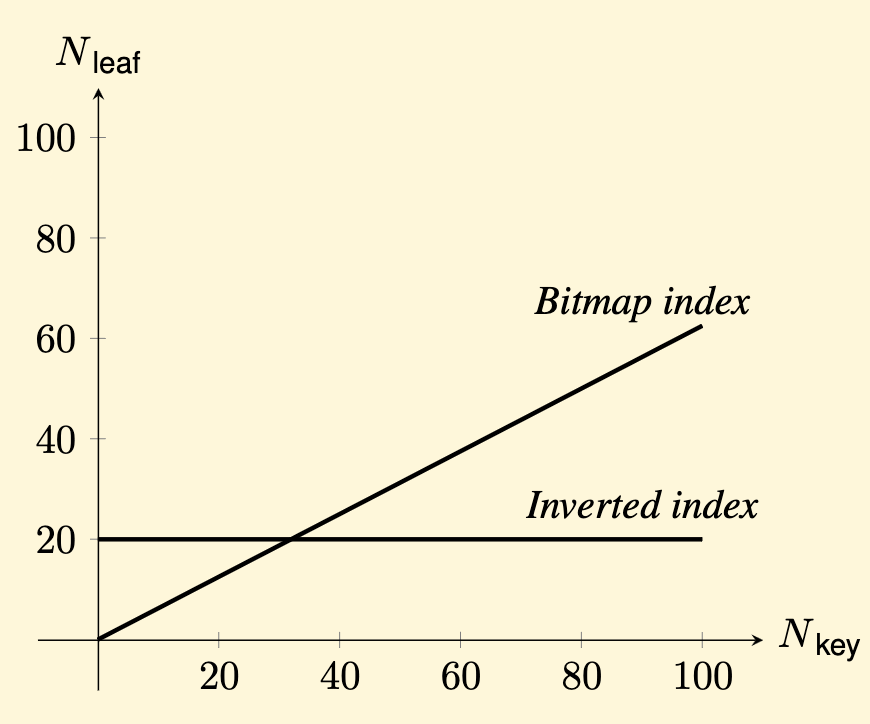
\includegraphics[width=0.5\linewidth]{img/bitmap_vs_inverted.png}
    \caption{Memory usage of bitmap and inverted indexes.}
    \label{fig:bitmap-vs-inverted}
\end{figure}

\subsection{Multidimensional Data Organization}

Multidimensional (or spatial) data is used to represent geometric objects and their position in a multidimensional space. Each record represents a point in the space, has a certain number of attributes that each represent the coordinates. Some common queries in multidimensional datasets are searching for points that fall within a specified rectangular area, and searching for a point's nearest neighbor(s). A typical organization with a B$^+$-tree may not be a good solution, since it does not capture ``closeness'' among points on more than one attribute at a time (the one chosen as key).

A way to solve this issue is to partition the space into areas with the same amount of points, so that each partition can be mapped to a separate page and allow quick retrieval of points that are spatially close together. Consider the dataset represented in Figure \ref{fig:multidim-start}, and suppose that pages have a capacity of 2. The data space is first divided choosing a division value $d$ on one coordinate, so that all points whose attribute value for that coordinate is less than $d$ are inserted into a page, those with a higher value are inserted into the other one. $d$ is usually chosen as the half of the range or the median value. The first split is in Figure \ref{fig:multidim-index} (a), done on the $x$ axis. If the partitions are still too big to fit into pages, then a split is repeated considering another axis (Figure \ref{fig:multidim-index} (b)). The splits continue alternating axes until each partition contains a small enough number of records. All the records belonging to the same partition will be found in the same page.

\begin{figure}[ht]
\centering
\begin{minipage}{0.49\textwidth}
    \centering
    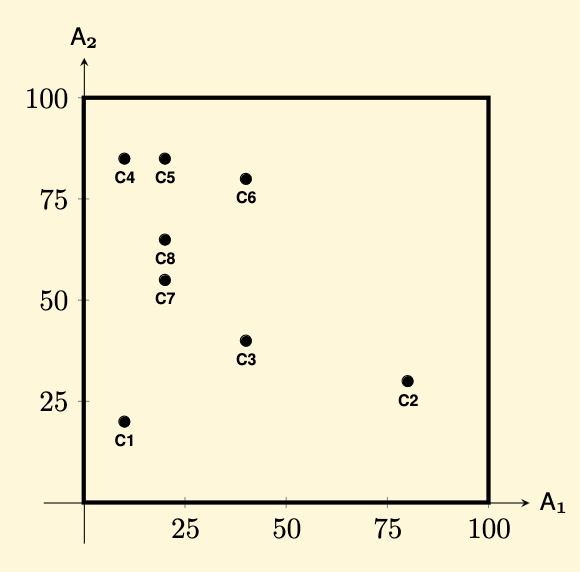
\includegraphics[width=0.5\linewidth]{img/multidim_start.png}
    \caption{Graphical representation of a two-dimensional dataset.}
    \label{fig:multidim-start}
\end{minipage}
\hfill
\begin{minipage}{0.49\textwidth}
    \centering
    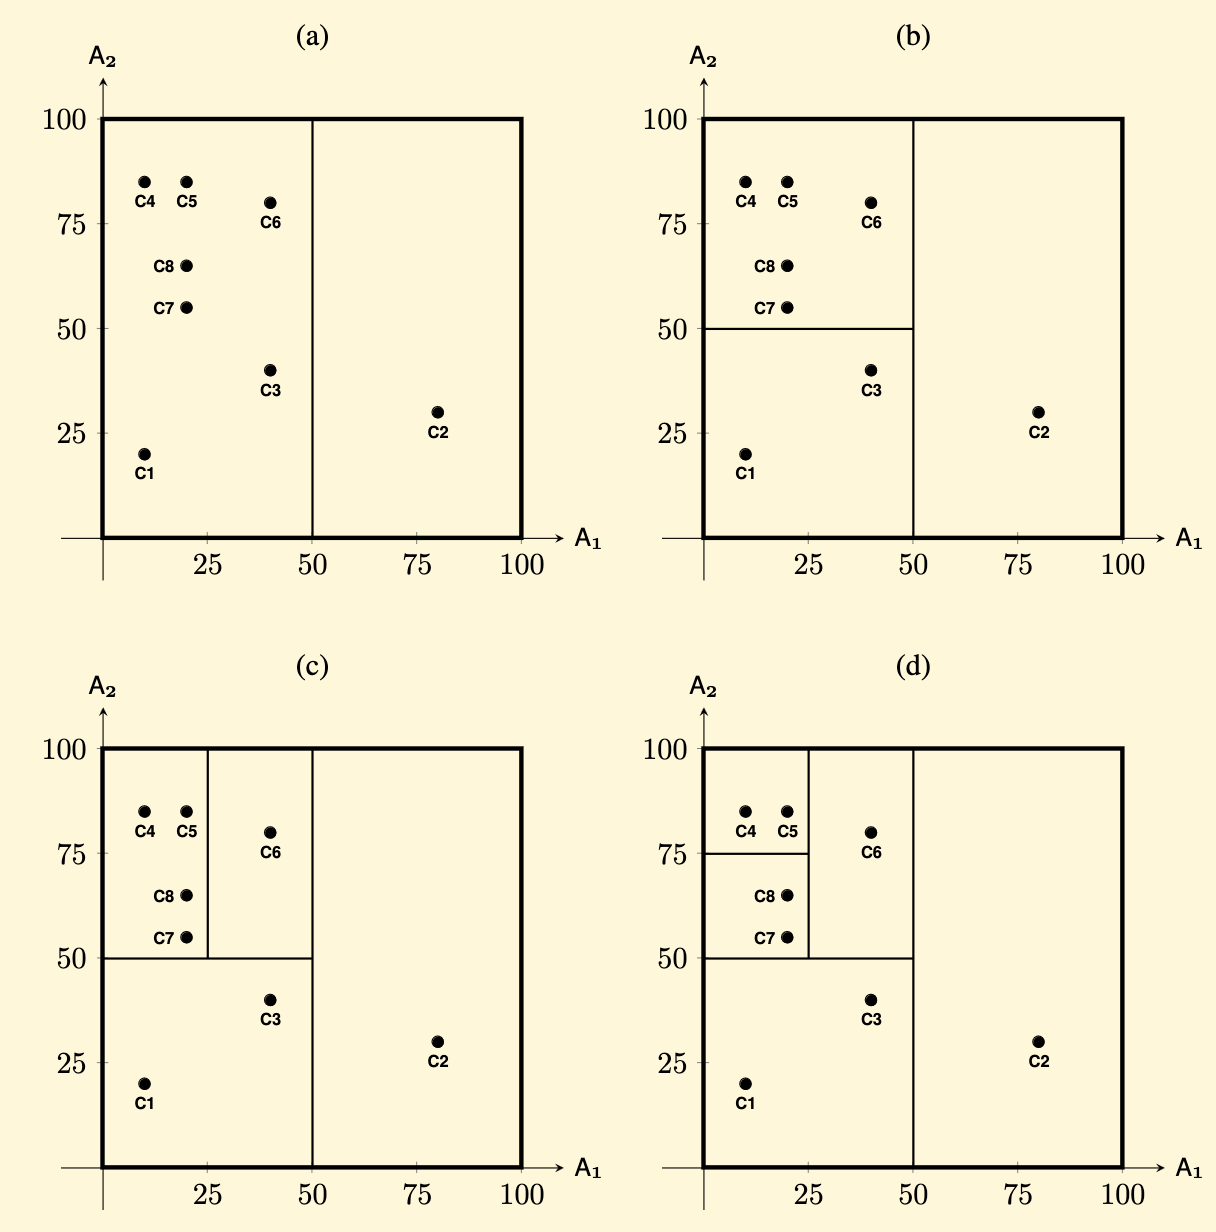
\includegraphics[width=\linewidth]{img/multidim_index.png}
    \caption{Division of the space into partitions.}
    \label{fig:multidim-index}
\end{minipage}
\end{figure}

\subsubsection{G-trees}

G-trees are the data structure used to store multidimensional indexes, where each partition is identified by a \textbf{partition code}. As the space is partitioned, a sort of ``decision tree'' is built, where each node corresponds to an attribute test condition, alternating the attributes at each level. Partition codes are assigned as follows:
\begin{itemize}
    \item The initial, intact, region is identified by the empty string;

    \item After the first split, the two partitions produced are identified with the strings ``0'' and ``1';

    \item When each partition of the previous step is split along the other axis, the new partitions will be ``00'' and ``01'', and ``10'' and ``11'', and so on.

    \item In general, when a partition $R$ is split, the subpartitions will have a code that is equal to the code of the parent and 0/1 appended at the end.
\end{itemize}
Each partition code is then padded so that they all reach $M$ bits, where $M$ is the maximum number of splits made. The G-tree stores these codes like a B$^+$-tree, where the leaves contain all the codes and the internal nodes alternate pointers to leaves and duplicate keys.
\begin{figure}[ht]
    \centering
    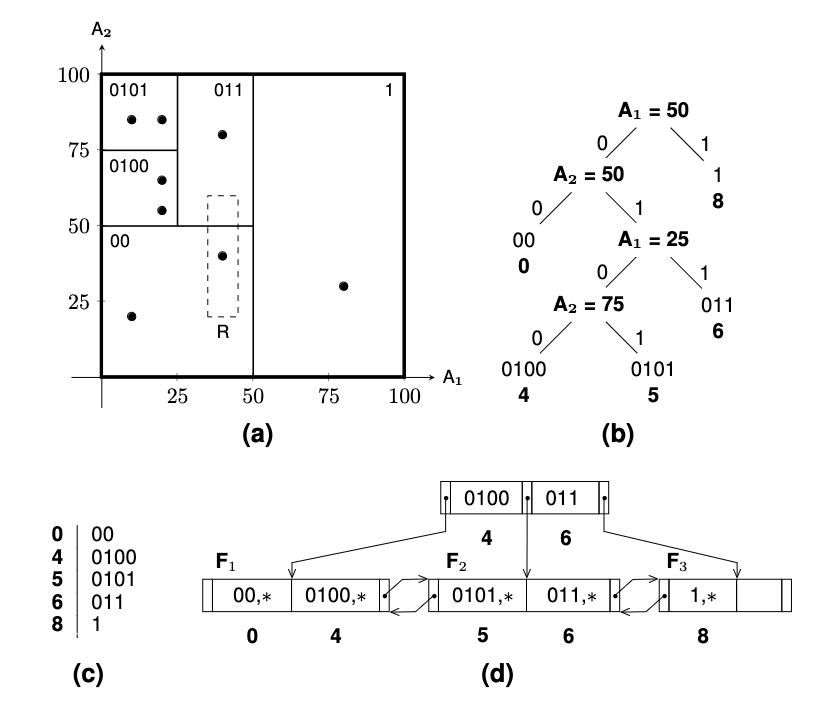
\includegraphics[width=0.5\linewidth]{img/G-tree.png}
    \caption{Example of partition coding.}
    \label{fig:G-tree}
\end{figure}
After the tree has been constructed, point search, insertion, deletion, and spatial range search can be done efficiently. To search a point $P$ with coordinates $(x, y)$, the partition code of the point is retrieved (if it is present), and the code is then used to search in the G-tree.

Range search is done by specifying a range for each axis. The search starts by identifying the lower left and upper right vertices of the rectangle area; the G-tree is searched for the nodes that contain these vertices, and for each leaf between them, the elements are searched, selecting all leaves that directly intersect with the search region.

For point insertion, first the G-tree is searched to find the partition that should contain the point; then, if that partition/leaf is not full, the point is simply inserted, otherwise, the partition must be split into two. Each partition is associated with the correct partition code, and if needed (the split adds a new level to the split tree) all other codes' padding is adjusted. The points in the original partition are distributed between the pages referred by the two leaves accordingly, and the parent node is updated with the new pointer and the duplicate key. If an overflow happens in the parent node, the same procedure seen for B$^+$-trees happens.

To delete a point, it is first searched in the G-tree, and the record is deleted. If the partition becomes empty, its code is removed from the tree. If the partition is the result of a split, and it can be merged with its sibling, then the merge is done and the two partition codes are replaced by the partition code of their parent.